\documentclass[letterpaper,10pt,serif,titlepage, onecolumn, compsoc]{IEEEtran}
\usepackage{graphicx}                                        
\usepackage{amssymb}                                         
\usepackage{amsmath}                                         
\usepackage{amsthm} 

\usepackage{alltt}                                           
\usepackage{float}
\usepackage{color}
\usepackage{url}

\usepackage{balance}
\usepackage[TABBOTCAP, tight]{subfigure}
\usepackage{enumitem}
\usepackage{pstricks, pst-node}

\usepackage{geometry}
\geometry{textheight=8.5in, textwidth=6in}

\usepackage{caption}
\usepackage{placeins}

\title{Team LibNav \\ Spring Midterm Progress Report \\ CS Senior Capstone \\ \vspace{2mm}\small CS461 (Fall 2016)}
\author{Authored by \\ Nathan Healea, Stephen Krueger, Matthew Zakrevsky}
\date{November 14, 2016}
\begin{document}

% Title page
\maketitle



% project purpose
\section*{Project Purpose}
Libnav's main purpose is to provide navigation assistance for patrons and visitors of Oregon State University’s Valley Library through the use of an interactive map. By using a start location and destination, Libnav will provide a navigation line through the multiple floors of the library to help guide users. Search for locations by attributes or name will help make finding a desired space or location an easier task. 

% Project Goal
\section{Project Goal}
Libnav’s goal is to make searching for and navigating to visitor’s destinations an easier and quicker task. Libnav will accomplish this through a web application that is mobile friendly and uncluttered by extra features. With a fully editable map, members of the library staff will be able to update locations and spaces as needed.  Libnav is designed to be portable and usable with both visitors and staff in mind, allowing for the application to be used for years to come. 


% Nathan Healea Section (NHS)
\section{Nathan Healea}

% NHS: Intel NUC (NUC)
\subsection{Intel NUC}
\subsubsection{Current Status}
Since the end of last term, the Intel NUC has not had any major work done on it. At the end of last term, we were able to fix the issue with the NUC not allowing us to connect to it. As the team started integrating the CAS login system, we were notified by OSU Network ID (ONID) that our URL was changed from libnav.engr.oregonstate.edu to fw-libnav.eecs.oregonstate.edu. 


\subsubsection{Problems that have impeded progress}
A change in URL raised some concerns with connecting to the application, but did not cause a problem that impeded progress.


\subsubsection{Solutions}
With the change in URL, we attempted to connect to the application which was successful. 

% User Interface
\subsection{User Interface}
\subsubsection{Current Status}
Since Spring Break, a lot of changes were made to the user interface. In the Librarian Administration Dashboard, a new view was developed for adding a user into the application to grant them access that consisted of a form, data table for view users, and a modal to alert the user of the status of the their request. The location forms also had a refactor done to them to add two new input fields to add a custom color and an option to display the location name or not. A toggle button was also added to all of the forms to hide locations on the map to make it easier to determine where to draw a location. When a location is being edited, the floor maps are automatically changed to the correct floor for the location being edited. A new view was added to display a location’s detail and location on the correct floor map. The navigation form had a new feature added that indicates to the user that the grid has been saved to the database and reloads the grid to the current floor being edited while reflecting the changes made.

In the front-end of the application, new features were added to the sidebar that allow a user to click on a location and have that location be highlighted on the map for the correct floor. This same function was implemented to the search results. The navigation block was refactored to move to the top of sidebar on larger screens, and to the bottom of the sidebar on smaller screen sizes. Tooltips were refactored to make them more visible, close automatically when the start and end buttons were clicked, and scroll if the location information exceed the height and width of the tooltip. 

\subsubsection{Problems that have impeded progress}
\begin{enumerate}
	\item No problems have impeded the progress of the user interface this term. Majority of the work has been minor bug fixes, with the exception of the detail and edit views. 
\end{enumerate}

\subsubsection{Solutions}
\begin{enumerate}
	\item No solutions needed to be applied.
\end{enumerate}

\newpage

\subsubsection{Images}
\begin{figure}[h!]
\centering
\captionsetup{justification=centering,margin=2cm}
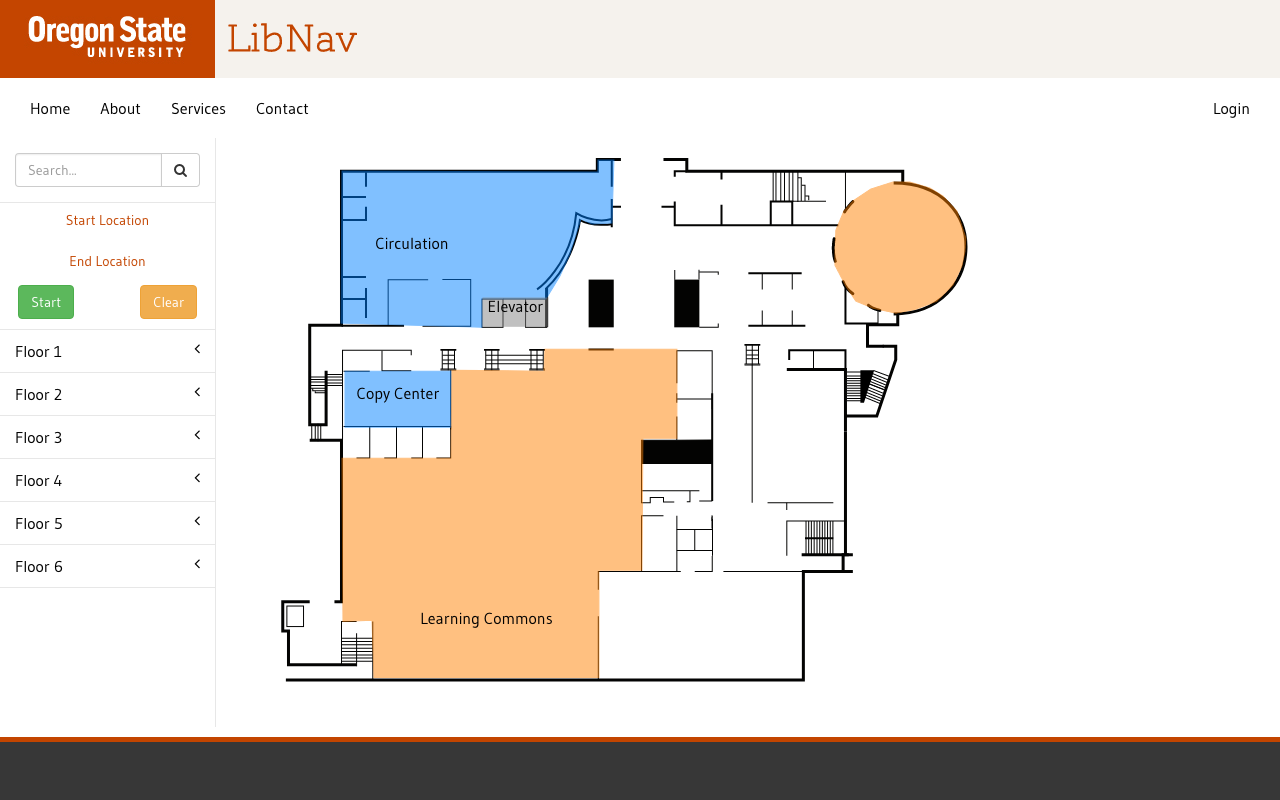
\includegraphics[width=0.90\textwidth,natwidth=1200,natheight=800]{images/main-page.png}
\caption{Interactive Map Layout}
\label{fig:method}
\end{figure}

\FloatBarrier
\begin{figure}[h!]
\centering
\captionsetup{justification=centering,margin=2cm}
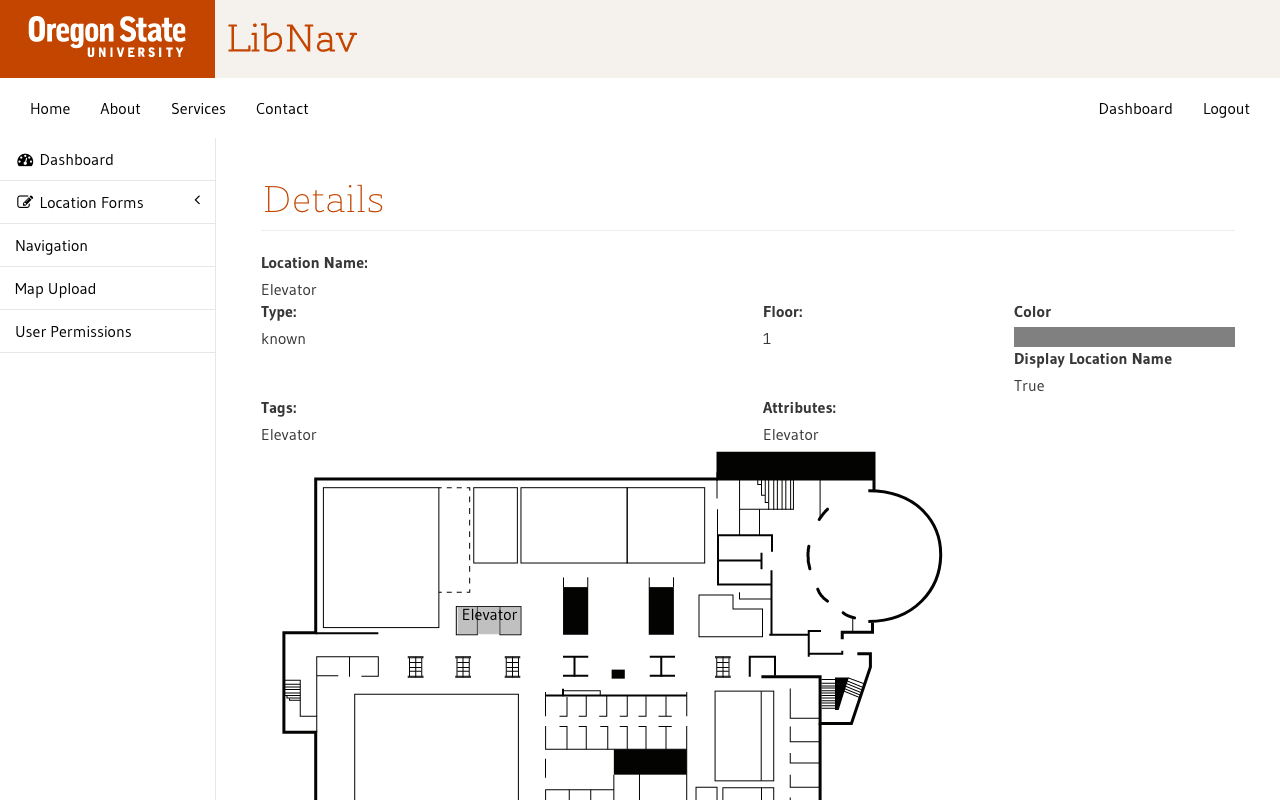
\includegraphics[width=0.90\textwidth,natwidth=1200,natheight=800]{images/detail-view.png}
\caption{Location Detail View}
\label{fig:method}
\end{figure}

\FloatBarrier
\begin{figure}[h!]
\centering
\captionsetup{justification=centering,margin=2cm}
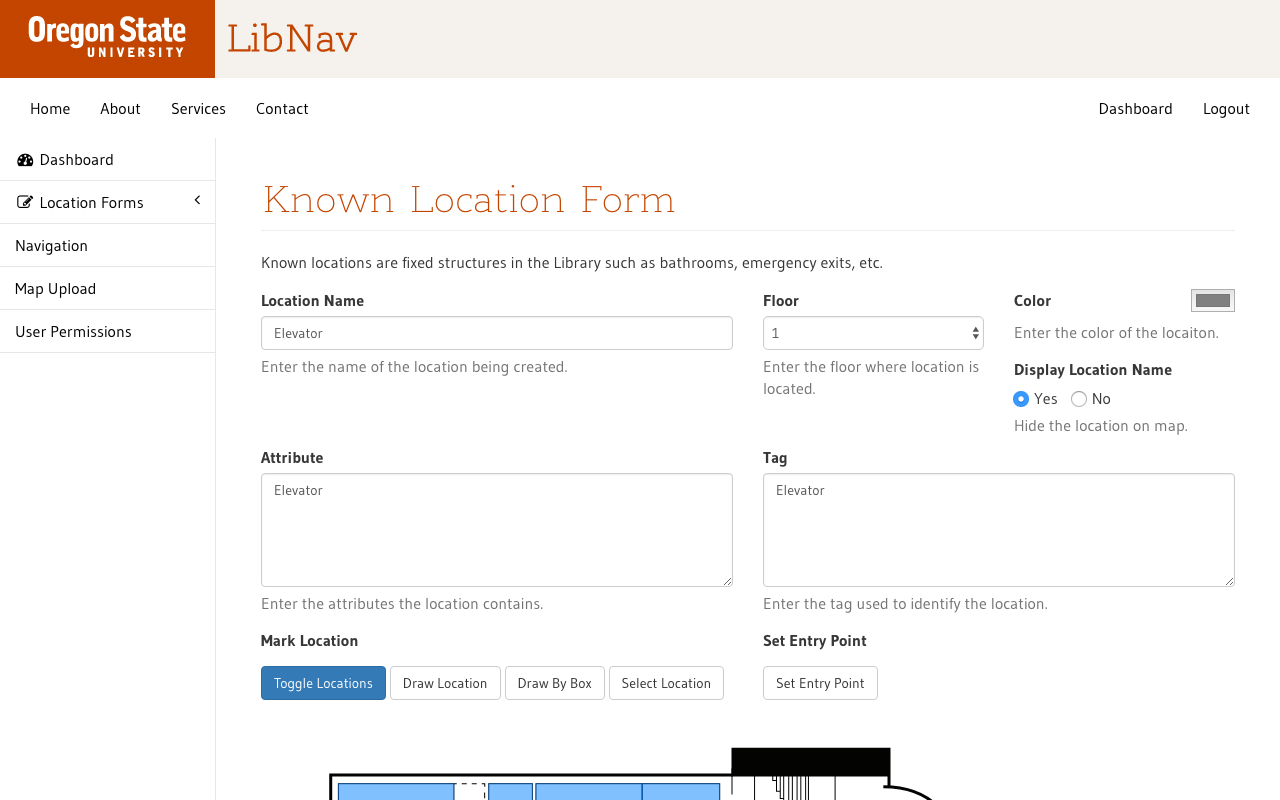
\includegraphics[width=0.90\textwidth,natwidth=1200,natheight=800]{images/editing-location.png}
\caption{Editing Location}
\label{fig:method}
\end{figure}

\FloatBarrier
\begin{figure}[h!]
\centering
\captionsetup{justification=centering,margin=2cm}
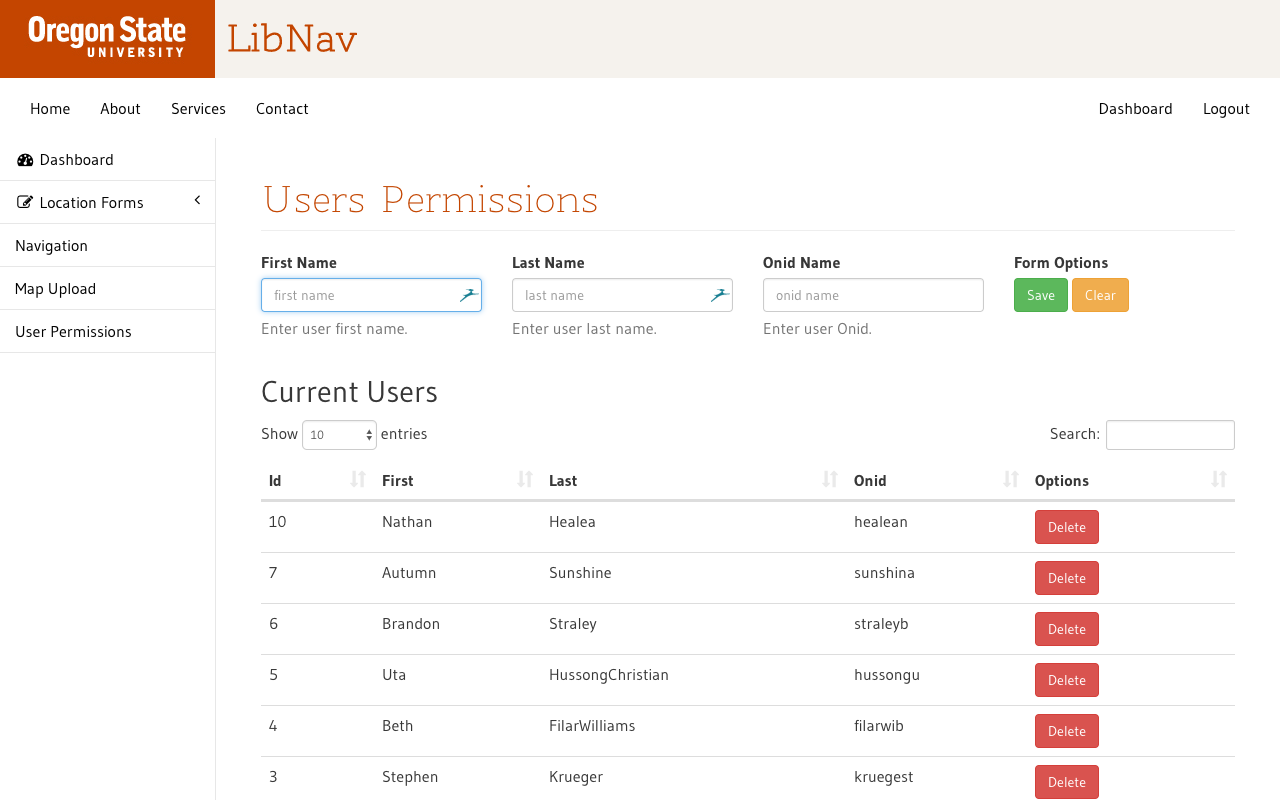
\includegraphics[width=0.90\textwidth,natwidth=1200,natheight=800]{images/user-permission.png}
\caption{User Permission View}
\label{fig:method}
\end{figure}

% Data Validation and Sanitation (DVS)
\subsection{Data Validation and Sanitzation}
\subsubsection{Current Status}
At the beginning of spring term, changes to the way locations are being saved into the database and stored in the global variables meant that a refactor to the data validation and sanitization had to be made. Instead of location’s attributes and tags being passed as an array of strings in the location data object, is now a stringified array that is still part of the location data object. This change  was made to help cut down on database querying, which will be explained in more detail later in the database section. 

New editing functionality was added so that location data objects are now parsed out and fill input fields for corresponding location types utilizing the same location forms for creating a new location. When the edits are completed, the same validation for a new location is used for an edited location. Also, new validation rules have been added for the color input along with the display of the location name input. 

\subsubsection{Problems that have impeded progress}
\begin{enumerate}
	\item  One problem that impeded the progress was the design of our application and how tags and attributes were being saved into our database. Complex loops for database inserts made updating a location nearly impossible. 
\end{enumerate}

\subsubsection{Solutions}
\begin{enumerate}
	\item To fix this problem, a refactor was done, as mentioned above, to improve how locations were stored in the database. This made validating, editing, and updating a location much easier and cleaner. 
\end{enumerate}

% User Authentication and Sessions (UAS)
\subsection{User Authentication and Sessions}
\subsubsection{Current Status}
Over Spring Break, work was completed to get Central Access Server (CAS) working within our project. As mentioned above in the NUC section, we were notified that our URL was changed and after some back and forth with Oregon Network ID (ONID), we confirmed that the NUC’s new URL was fw-libnav.eecs.oregonstate.edu. Once this was figured out and ONID granted our application access to use CAS, a refactor of our user.js controller was needed. When the user clicks the login link on the homepage, they are redirected to the CAS service at OSU. Then, once a valid username and password has been entered, CAS sends a token back to our application. A request from our application is made using the token to verify our application. Once verified, the user’s CAS information is sent to our application, parsed out, and the ONID is checked against ONIDs in our application database for access. 

\subsubsection{Problems that have impeded progress}
\begin{enumerate}
	\item One problem that has impeded our progress was the fact the the NUC was not able to be accessed via a URL.
    \item The second was that we needed to have our application registered with ONID.
\end{enumerate}

\subsubsection{Solutions}
\begin{enumerate}
	\item The first problem was fixed at the end of winter term. ONID verified that the URL had been changed.
    \item To resolve the second problem, our team contacted ONID to get LibNav registered to be able to use CAS.
\end{enumerate}

%Stephen Section (SS) 
\section{Stephen Krueger}

% SS: Navigation (NAV)
\subsection{Navigation}
\subsubsection{Current Status}
The navigation system is for all intents and purposes completed. Single floor navigation between two locations works very well and meets all requirements. Recently two floor navigation was implemented and is working. The navigation path line between two locations has been visually updated. Instead of rectangles it is now made up of little circles which most users should be familiar with if they have used google maps for walking directions. We also added pins to mark the starting location and the end location. 

\begin{figure}[h!]
\centering
\captionsetup{justification=centering,margin=2cm}
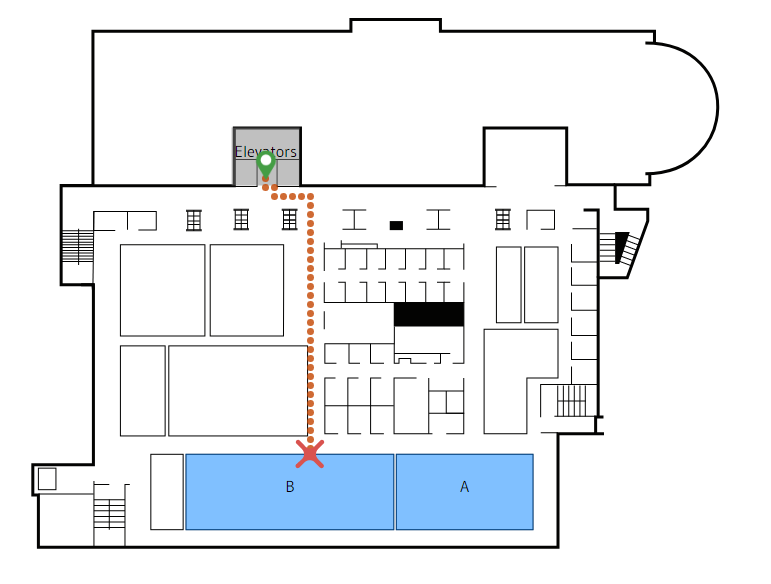
\includegraphics[width=1\textwidth,natwidth=771,natheight=584]{images/line.png}
\caption{Navigation Line}
\label{fig:method}
\end{figure}

Saving the grid to the database was re-factored and now works much better. We store a stringified json of the whole grid instead of having a table to store the grid points. When you make changes on the grid on the dashboard page it will update on save without having to reload the page. We also added entry points to the grid map, so that the admin can make sure that all the rooms on the grid are connected and navigation on the home page will work for every location. 

\subsubsection{Problems that have impeded progress}
\begin{enumerate}
\item I had to wait for the refactoring of our database to implement two floor navigation. This is because the way we were going to be receiving the location and grid data from the database was going to change with the refactor. Any implementation done before that would have had to be re-written. 
\end{enumerate} 

\subsubsection{Solutions}
{\begin{enumerate}
\item Currently two floor navigation only works using the elevators. We would like to have the option to navigate between two floors using stairs as well. We think this would be a great option for a campus that is so health-orientated. The library could use this option to promote a healthier alternative. It could also be used to control traffic by defaulting to one option or the other. It’s not a huge change in the code but it would require UI updates so we decided to hold off until after the spring Expo.
\end{enumerate}}



% SS: Map Upload (ML)
\subsection{Map Upload}
\subsubsection{Current Status}
The map upload is functional but not perfect. Currently the path to the images folder needs to be configured depending on the setup of the server so it’s not a perfect solution. It does work however. You can take a map and upload it to the images folder. It overwrites the current map and the new map will be loaded and ready to be used.

There is still some work we would like to do with the map upload. This includes having an image preview. After the map is uploaded and before it is saved we would like to have a test environment so that the admin can check and make sure all the rooms are selectable. We would also like to implement some security measures so that only SVG files can be loaded. 

\subsubsection{Problems that have impeded progress}
\begin{enumerate}
\item I had to try multiple node middle-ware packages in order to get the map upload to work correctly. Some of the packages had poor documentation and it wasn’t till I found a stack overflow comment that I figured out that its usage was depreciated and wouldn’t work with our current framework. 

Due to the nature of the implementation, we can’t redirect on success. So we simply provide a success message and a link to return the user to the dashboard. 
\end{enumerate}


\subsubsection{Solutions}
\begin{enumerate}
\item This was incredibly frustrating to deal with and eventually I just used expressJS, an ajax call, and basic javascript to do it. I figured out how to use the body-parser that comes with expressJS to successfully send files in the body of the ajax request. Once I was able to do that I simply got the file and moved it to the correct location on the server. Luckily html-5 inputs now make it easy to get the file from the input field. 
\end{enumerate}


% SS: Database
\subsection{Database}
\subsubsection{Current Status}
The database is currently set up and in its final form. Writing location data, grid data, and user session data to the database all works. The queries to return that data from the database are all functional. The database is also currently setup to hold the admins custom drawn locations and grids. We can get the data points back from the database and re-draw those locations on the map and re-draw the saved grid. We can also successfully update locations and grid data through async requests allowing for a smooth user experience. 

\subsubsection{Problems that have impeded progress}
\begin{enumerate}
\item The location data was originally stored as individual data points and when we went to pull the data and loop through the points it was painfully slow. We decided that we would need to refactor the database to store grid and location objects as a json objects.
\end{enumerate}

\subsubsection{Solutions}
\begin{enumerate}
\item The tables that were used to store the individual data points were deleted. Instead we store the data points in a json object. We will then stringify the object of points and store the string in the database. Now when we pull out the points it's already in an nice iterable object format.
 The tables that were used to store the individual data points were deleted. Instead we store the data points in a json object. We will then stringify the object of points and store the string in the database. Now when we pull out the points it's already in an nice iterable object format.
One other change is that we do the major queries on page load now. So when the site first loads it grabs a JSON of all the locations and all of the grids and stores them in global variables that are used throughout the application. Substituting a bunch of smaller calls for a few large calls means that the database is less stressed and improved performance of the application overall. It also made the code much more readable than before.
\end{enumerate}

%Matthew\
\section{Matthew Zakrevsky}
\subsection{Software Framework}
\subsubsection{Current Status}
As it currently stands the web framework that we are using is the Express framework previously discussed in our design  and requirements documents. This framework controls the routing of the web pages and is fully functional with the bootstrapping, mysql post and get  queries. The use of Express has allowed us to use routes to move between the various web pages without error, .The  framework has been meeting our needs though previously there were some minor problems in how data was being retrieved from the database and how frequently this data was being retrieved. This had to do with the need to use asynchronous ajax calls. These database calls were removed and instead a single monolithic json object is populated on page load. This monolithic object is parsed instead of making multiple calls for the same data.

\subsubsection{Problems that have impeded progress}
\begin{enumerate}
\item need to use asynchronous ajax calls to use the mysql controller
\end{enumerate}


\subsubsection{Solutions}
\begin{enumerate}
\item As a team we decided that it would be best to remove as many of the asynchronous calls from the project as we could. The purpose of this was to the program run more efficiently when many users are accessing the program at once. By making one call to the database on loading the main page, the project makes use of a single monolithic json object that is parsed by the search, the drawLocations function, and the tooltips on the front end rather than querying the database every time we need the same information. This decreases the amount of traffic through the application.
\end{enumerate}

\subsection{SVG Rendering and Map Drawing }
\subsubsection{Current Status}
SVG rendering is complete as per the instructions provided by our client. There have been no major problems as much as additions that the client would like to see, such as the ability to toggle space names on and off or the ability to change the color of the locations being drawn on the map. The biggest changes to this part of the project the were the Tooltips and the functionality/design of these element. These tooltips are now on-click events and contain buttons for navigation and a button to close the tooltip. An additional drawing function was made to ease the amount of free handed drawing that needs to be done. This additional drawing function allows the staff to click where they would like the top left corner and where they would like the bottom right corner and will derive a rectangle from that information.

\subsubsection{Problems that have impeded progress}
\begin{enumerate}
\item Changing drawing with specific colors and name display
\item Changes to the tooltip to make them on click to fix how other devices handle touch based \item 	commands, including selecting a location as the start or end location for navigation.
\item The ability to draw cleaner shapes not within the svg file.
\end{enumerate}

\subsubsection{Solutions}
\begin{enumerate}
\item The solution to these requirements provided to use by our clients were solved by adding two more options to the locations table. If these values are not null then the code will know what to do to make sure that they are displayed correctly. The color is simply passed to the D3.append call that creates the shape as an attribute. The name on the other hand has to be placed separately with a center location derived from the points of the shape to be drawn.
\item The tool tip is built upon dynamically created html divs that are styled with the handlebars system that we are using for views. These Tooltip are now on-click events opposed to  on-hover events. This is because on mobile devices on-click functions are treated  the same as on- hover. With this we had to make a change such that we could make use of only on-click functions, thus on-click to open the tooltip and additional buttons to navigate or close the tooltip. These tool tips also close when navigation begins. This was more of usability choice than an actual problem with the functionality.
\item The last problem that makes life easier for the clients and anyone who is creating spaces in the application. Basically based on the two points, the last two point are derived with a combination of x,y coordinates before combining this into the . This not only makes cleaner shaped but ergonomically this requires less movement from the mouse which is tiring for a long period of time.
\end{enumerate}

\subsection{Search Functionality }
\subsubsection{Current Status}
Since the beginning of the term the major changes made to the search functionality have been the ability to change the  map to a different floor  when a result is clicked, highlighting a result on the map, and a refactor to the code to match how names, tags, and attributes are matched to the search string. This functionality is otherwise complete with a small bug that occurs when a result on a different floor is selected, specifically it does not highlight the object after the new floor is loaded. Additionally over the course of the term time was spent tuning the search function so that it would match more accurately
\subsubsection{Problems that have impeded progress}
\begin{enumerate}
\item Map change when the search location is clicked.
\item Highlighting the searched object on the map
\item Code refactor to search the monolithic json object of locations rather than getting all tags, attributes, and names from the database.
\item Tuning the database to accurately match the contents of the monolithic JSON object.
\end{enumerate}
\subsubsection{Solutions}
\begin{enumerate}
\item This problem was solved with the introduction of a listener which is used to perform some action whenever the location in the search results field. THis in combination with the loadMap function from when we load maps with any of the drop down menus.
\item Highlighting was extended to use the code that is used to highlight a space when it is selected from the floor drop down. There is a bug where it does not show highlight when a new floor is loaded but after discussion with the client the ability to just click the space in the search results again is fine. 
\item This problem stems from a refactor made during spring break where as a team it was decided that we would create monolithic object with all location data, populated when the web page loads. This was solved by changing what and how Fuse.js searched the JSON object. The changes made were redefining the scope of the keys to match the key-value pairs in the monolithic JSON object 
\item The solution to this project was to create a series of if else statements that changed set the minimum number of matched characters and  the weighted results returned from the search.

\end{enumerate}


\newpage
\end{document}
